\chapter{Annotated Bibliography of Seminal Works}
\label{app:annot}

The framework developed in this monograph for quantifying ion energy flux across plasma sheaths draws on seven interlocking bodies of literature: kinetic and fluid theory of the sheath and presheath; the definition and measurement of ion energy flux at bounding surfaces; non-perturbative laser-induced-fluorescence (LIF) diagnostics of the ion velocity distribution function (IVDF); Thomson-scattering diagnostics of the electron population adjoining the sheath; the mathematics of ill-posed inverse problems used to reconstruct distribution functions and profiles from noisy data; erosion and lifetime studies in Hall-effect thrusters; and plasma-wall interaction (PWI) in magnetically confined fusion devices. This appendix is not an exhaustive survey; it selects works judged most seminal to the chain of reasoning used in the main text --- from the Bohm criterion, through the definition of the energy-resolved ion flux $\Gamma_{E}$, to its diagnostic reconstruction and consequences for wall erosion. Entries are grouped by theme, each opening with a paragraph fixing notation and the governing equation the theme's works refine. No cited or plotted quantity here should be read as a measurement by the present authors; all figures are schematic. Notation is fixed throughout: $T_{\mathrm{e}}$ and $T_{\mathrm{i}}$ denote electron and ion temperature in energy units, $n_{\mathrm{e}}$ and $n_{\mathrm{i}}$ the corresponding number densities, $\lambda_{\mathrm{D}} = \sqrt{\varepsilon_{0} T_{\mathrm{e}}/n_{\mathrm{e}} e^{2}}$ the electron Debye length, $u_{\mathrm{B}}$ the Bohm speed, $\Gamma_{E}$ the ion energy flux density, and $f_{\mathrm{i}}(v)$ the ion velocity distribution function.

\section{Sheath Theory and the Bohm Criterion}
\label{app:annot:sheath-theory}

The plasma sheath is the thin, positively net-charged, quasi-static boundary layer through which a bulk plasma matches its potential to a much lower, wall-imposed value. Its existence and monotonicity depend on the Bohm criterion, bounding the ion speed entering the sheath from below. For a one-dimensional, planar, collisionless system with cold ions ($T_{\mathrm{i}} \to 0$) accelerated through a quasi-neutral presheath and Boltzmann-distributed electrons at temperature $T_{\mathrm{e}}$, energy conservation for a fluid ion element gives
\begin{equation}
\tfrac{1}{2} m_{\mathrm{i}} u^{2}(x) = \tfrac{1}{2} m_{\mathrm{i}} u_{0}^{2} + e\bigl[\phi_{0} - \phi(x)\bigr],
\label{eq:annot:ionenergy}
\end{equation}
where $u_{0}$ is the ion speed at the sheath edge ($\phi_{0} \equiv \phi(x{=}0)$) and $\phi(x) \le \phi_{0}$ for $x>0$. Steady-state ion continuity, $n_{\mathrm{i}}(x)\,u(x) = n_{\mathrm{e}}(0)\,u_{0}$, combined with the Boltzmann relation $n_{\mathrm{e}}(x) = n_{\mathrm{e}}(0)\exp\!\bigl[e(\phi(x)-\phi_{0})/T_{\mathrm{e}}\bigr]$ and Poisson's equation,
\begin{equation}
\frac{\mathrm{d}^{2}\phi}{\mathrm{d}x^{2}} = -\frac{e}{\varepsilon_{0}}\bigl[n_{\mathrm{i}}(x) - n_{\mathrm{e}}(x)\bigr],
\label{eq:annot:poisson}
\end{equation}
is linearised about $\phi = \phi_{0}$ to demand a monotonically increasing space-charge density into the sheath, yielding the Bohm criterion
\begin{equation}
u_{0} \ge u_{\mathrm{B}} \equiv \sqrt{\frac{T_{\mathrm{e}}}{m_{\mathrm{i}}}},
\label{eq:annot:bohm}
\end{equation}
with equality defining the marginal (cold-ion, collisionless, unmagnetized) case. The works below extend this result across warm-ion, kinetic, magnetized, multi-species, and collisional regimes, all germane to the flux estimator constructed in Chapter~3.

The kinetic formulation of the presheath and its consistency with the fluid Bohm criterion is established by \cite{ref0001}, whose treatment of ion trapping, the low-velocity ion tail, and the sheath-edge singularity structure is the clearest statement of why a monotonic potential drop demands Eq.~\eqref{eq:annot:bohm} rather than merely permits it. A synthesising review of the criterion's domain of validity, generalisations to multiple ion species and non-monotonic potentials, and historical development is given by \cite{ref0004}, the principal tutorial reference and source of terminology used throughout. The companion electron-sheath problem --- relevant when the wall is electron-attracting (biased near or above the plasma potential, e.g. via strong electron emission), exchanging the roles of the light and heavy species in Eq.~\eqref{eq:annot:poisson} --- is developed in \cite{ref0006}. The exact collisional generalisation, retaining ion-neutral friction to all orders in the presheath momentum balance, is derived in \cite{ref0009}, underlying the finite-collisionality correction in the flux estimator's error budget; a complementary fluid treatment of low-pressure sheath formation is given in \cite{ref0024}.

A second cluster addresses the coherence of the plasma-wall transition as a boundary-value problem. The general transition, of which the Bohm criterion is the marginal boundary condition at the quasi-neutral/space-charge interface, is reviewed comprehensively in \cite{ref0013}. A candid assessment of the persistent disagreements surrounding the transition --- the location of the sheath edge, the ion source term, and the equality versus strict-inequality form of Eq.~\eqref{eq:annot:bohm} --- is offered in \cite{ref0015}, cited here as the clearest statement of why the flux estimator of Sec.~\ref{app:annot:ion-energy-flux} must carry an explicit treatment of presheath uncertainty.

Magnetized and multi-fluid generalisations form a third cluster essential to the anisotropic flux geometry discussed in the main text, since every later application involves a magnetized sheath in which ion flow is not purely one-dimensional. The magnetized extension, the Bohm--Chodura criterion,
\begin{equation}
u_{\parallel,0} \ge u_{\mathrm{B}}\cos\theta_{B},
\label{eq:annot:bohmchodura}
\end{equation}
where $u_{\parallel,0}$ is the ion speed parallel to a magnetic field incident at angle $\theta_{B}$ to the surface normal, and a wider magnetic presheath accelerates ions to satisfy Eq.~\eqref{eq:annot:bohmchodura} before the thinner electrostatic sheath is reached, is formalised in \cite{ref0017}, adopted here as the boundary condition for all magnetized-source case studies. A two-fluid formulation spanning the presheath and space-charge sheath self-consistently, retaining a finite ion-pressure term omitted from Eq.~\eqref{eq:annot:ionenergy}, is developed in \cite{ref0023}, providing the warm-ion correction used whenever $T_{\mathrm{i}}/T_{\mathrm{e}} \gtrsim 0.1$.

\section{Ion Energy Flux at the Plasma Boundary}
\label{app:annot:ion-energy-flux}

The central diagnostic quantity of this monograph is the energy flux density carried by ions across the sheath onto a bounding surface. Given $f_{\mathrm{i}}(v)$, normalised such that $\int_{0}^{\infty} f_{\mathrm{i}}(v)\,\mathrm{d}v = n_{\mathrm{i}}$, the one-sided particle and energy fluxes at the wall are
\begin{align}
\Gamma_{\mathrm{i}} &= \int_{0}^{\infty} v\, f_{\mathrm{i}}(v)\, \mathrm{d}v, \label{eq:annot:gammai}\\
\Gamma_{E} &= \int_{0}^{\infty} \tfrac{1}{2} m_{\mathrm{i}} v^{2}\, v\, f_{\mathrm{i}}(v)\, \mathrm{d}v, \label{eq:annot:gammaE}
\end{align}
so the mean ion impact energy is $\langle E_{\mathrm{i}} \rangle = \Gamma_{E}/\Gamma_{\mathrm{i}}$. In the collisionless, cold-source limit with monoenergetic acceleration through a sheath potential drop $\Delta\phi$, Eq.~\eqref{eq:annot:gammaE} reduces to $\Gamma_{E} \approx \Gamma_{\mathrm{i}} \bigl(\tfrac{1}{2}T_{\mathrm{e}} + e\Delta\phi\bigr)$, where $\tfrac{1}{2}T_{\mathrm{e}}$ is the presheath contribution from ions already moving at $u_{\mathrm{B}}$. Three failure modes recur below: collisions broaden $f_{\mathrm{i}}(v)$, redistributing $\Gamma_{E}$ into a lower-energy shoulder without changing $\Gamma_{\mathrm{i}}$; a bias-waveform period comparable to the ion transit time modulates $\Delta\phi(t)$, making $\Gamma_{E}$ a transit-time-weighted average; and deviation of the bulk electrons from a single Maxwellian rescales $u_{\mathrm{B}}$, coupling the presheath term to the shape of $f_{\mathrm{e}}(v)$.

The dependence of surface processing rates on the full energy-resolved flux is modelled explicitly in \cite{ref0074}, coupling an ion energy flux-dependent etch-rate law to sheath kinetics; the law is structurally identical to the erosion integral of Eq.~\eqref{eq:annot:erosion} introduced later, with $Y(v)$ replaced by an energy-dependent reaction probability. A dedicated sensor for in-situ, real-time measurement of $\Gamma_{E}$ is reported in \cite{ref0075}. The ion-bombardment contribution to total heat flux on a wafer surface in an inductively coupled etch tool is isolated in \cite{ref0080}, separating the energy-flux term from neutral-radical and photon contributions to the measured load. Ion-neutral collisions' effect on the weakly collisional sheath, and the resulting reduction of the energy-resolved flux relative to the collisionless prediction, is quantified in \cite{ref0077}. A data-driven closure for heat flux in electrostatic plasma phenomena is developed in \cite{ref0101}.

The sheath formation criterion and resulting ion flux for a non-Maxwellian bulk electron population --- generalising the Boltzmann relation underlying Eq.~\eqref{eq:annot:bohm} to an arbitrary $f_{\mathrm{e}}(v)$, and hence effective $u_{\mathrm{B}}$ --- is derived in \cite{ref0090}. The power balance of a fusion reactor, in which ion, neutron, and radiative energy fluxes onto the first wall and divertor close a reactor-scale energy accounting, is formulated in \cite{ref0093}, situating $\Gamma_{E}$ within a device-integrated budget revisited in Sec.~\ref{app:annot:fusion-pwi}.

A review of tailored ion energy distributions on biased plasma electrodes --- waveform-tailoring, electrical-asymmetry-effect, and pulsed-bias techniques by which a narrow, controllable $f_{\mathrm{i}}(v)$ can be imposed at a processing surface --- is given in \cite{ref0105}, and the specific realisation of such tailoring at an ultra-low bias frequency, with the resulting IEDF resolved experimentally, is reported in \cite{ref0106}.

\section{Laser-Induced Fluorescence Diagnostics of the Ion Velocity Distribution Function}
\label{app:annot:lif-ivdf}

Laser-induced fluorescence provides the primary non-perturbative route to $f_{\mathrm{i}}(v)$ used to close Eqs.~\eqref{eq:annot:gammai}--\eqref{eq:annot:gammaE} experimentally. A narrow-linewidth, tunable laser is scanned across a Doppler-broadened absorption line of a metastable or ground-state ion; the fluorescence intensity versus detuning $\Delta\nu$ is proportional to the projection of $f_{\mathrm{i}}(v)$ onto the laser wavevector $\hat{\mathbf{k}}$, via $\Delta\nu = (\mathbf{k}\!\cdot\!\mathbf{v})/2\pi$. Requiring no material probe immersed in the sheath, the technique uniquely resolves $f_{\mathrm{i}}(v)$ within the sheath itself, at scales comparable to $\lambda_{\mathrm{D}}$, without perturbing the space-charge structure measured.

A direct, spatially resolved LIF observation of the ion velocity distribution function inside a plasma sheath, confirming the acceleration and narrowing of $f_{\mathrm{i}}(v)$ predicted by sheath theory, is reported in \cite{ref0329}. The foundational methodology for extracting quantitative ion distribution functions from LIF spectra, including deconvolution of instrumental and natural linewidth contributions, is established in \cite{ref0338}, with a general account of the technique's physical basis given in \cite{ref0300}. A xenon Hall-thruster implementation using diode-laser LIF is presented in \cite{ref0322}, and a broader methodological review of what IVDF measurements reveal about the underlying plasma physics is given in \cite{ref0347}. The application of planar LIF as a plasma-processing diagnostic, with discussion of instrumental error sources, is reviewed in \cite{ref0304}. Finally, the extension of planar LIF to a fully three-dimensional, tomographic reconstruction of $f_{\mathrm{i}}(\mathbf{v})$ in an electric-thruster plume, combining multiple line-of-sight LIF projections through a computed-tomography-style inversion, is demonstrated in \cite{ref0328}; this is the experimental counterpart of the inversion mathematics of Sec.~\ref{app:annot:inverse-problems}.

Table~\ref{tab:annot:diagnostics} collects the principal observable, its governing relation, and representative works from the themes covered so far.

\begin{table}[htbp]
\centering
\caption{Representative diagnostic and reconstruction approaches referenced in this appendix, grouped by the physical observable each targets. The table is a schematic organisational summary of the cited literature, not a compilation of measured values.}
\label{tab:annot:diagnostics}
\begin{tabularx}{\textwidth}{@{}l X l@{}}
\toprule
Approach & Physical observable & Representative works \\
\midrule
Point/planar LIF of $f_{\mathrm{i}}(v)$ & Doppler-resolved ion velocity distribution near the sheath edge & \cite{ref0329}, \cite{ref0338}, \cite{ref0322} \\
Tomographic LIF & Fully resolved $f_{\mathrm{i}}(\mathbf{v})$ in three velocity dimensions & \cite{ref0328} \\
Incoherent Thomson scattering & $n_{\mathrm{e}}$, $T_{\mathrm{e}}$ from the free-electron spectrum & \cite{ref0384}, \cite{ref0355} \\
Ion energy flux sensors & $\Gamma_{E}$ at a bounding surface, directly & \cite{ref0074}, \cite{ref0075} \\
Regularized inversion & $f_{\mathrm{i}}(v)$ or $n_{\mathrm{e}}(x)$ from noisy, line-integrated data & \cite{ref0677}, \cite{ref0683}, \cite{ref0692} \\
\bottomrule
\end{tabularx}
\end{table}

\section{Thomson Scattering Diagnostics of Sheath-Adjacent Plasmas}
\label{app:annot:thomson}

Incoherent Thomson scattering probes the electron population that sets the sheath potential drop through the Boltzmann relation of Eq.~\eqref{eq:annot:poisson}, by measuring the frequency-broadened spectrum of laser light scattered from free electrons. The scattered spectrum is governed by the dimensionless scattering parameter
\begin{equation}
\alpha \equiv \frac{1}{k\,\lambda_{\mathrm{D}}},
\qquad
k = \frac{4\pi}{\lambda_{0}}\sin\!\left(\frac{\theta_{\mathrm{s}}}{2}\right),
\label{eq:annot:thomsonalpha}
\end{equation}
where $k$ is the scattering wavevector set by the laser wavelength $\lambda_{0}$ and scattering angle $\theta_{\mathrm{s}}$. For $\alpha \ll 1$ (incoherent regime), the scattered power spectrum is directly proportional to the electron velocity distribution projected along $\hat{\mathbf{k}}$, giving simultaneous access to $n_{\mathrm{e}}$ and $T_{\mathrm{e}}$ without the assumptions required by electrostatic probes; for $\alpha \gtrsim 1$ (collective regime) the spectrum instead resolves plasma-wave resonances, a regime this monograph's measurements avoid via a sufficiently short probe wavelength.

The original methodology for extracting electron temperature and density from the Thomson-scattered spectrum of an optical laser beam is established in the classical work of \cite{ref0384}, treated here as the historical anchor of the technique. A modern review of Thomson-scattering diagnostics for chemically reactive and processing plasmas is given in \cite{ref0354}. An implementation targeting the electron properties of a Hall-effect thruster plasma, spatially resolving $n_{\mathrm{e}}$ and $T_{\mathrm{e}}$ across the acceleration region, is reported in \cite{ref0355}, providing a comparison point for the electron-side inputs to our flux estimator in magnetized propulsion plasmas; a companion measurement across the acceleration zone of a high-power, magnetically shielded Hall thruster --- the topology treated by the Bohm--Chodura condition --- is reported in \cite{ref0356}.

\section{Inverse Problems and Regularization for Distribution-Function Reconstruction}
\label{app:annot:inverse-problems}

Both LIF and Thomson-scattered spectra are line-integrated, noise-corrupted, finite-bandwidth projections of the underlying distribution function or profile of interest; recovering $f_{\mathrm{i}}(v)$, $n_{\mathrm{e}}(x)$, or a scattering-derived profile from such data is formally an ill-posed inverse problem in the sense of Hadamard, since the forward operator's inverse is unbounded and small data perturbations can produce unbounded reconstruction error. Tikhonov regularization addresses this by minimising a penalised functional,
\begin{equation}
\hat{f} = \operatorname*{arg\,min}_{f} \left\{ \lVert K f - d \rVert_{2}^{2} + \mu \,\lVert L f \rVert_{2}^{2} \right\},
\label{eq:annot:tikhonov}
\end{equation}
where $K$ is the forward (e.g. Abel, Doppler, or line-integration) operator, $d$ the measured data vector, $L$ a smoothing operator, and $\mu>0$ a regularization parameter chosen, e.g., by the L-curve or discrepancy-principle criteria to balance fidelity to $d$ against solution smoothness.

A direct application of Tikhonov-regularized inversion to a tomographic laser-absorption problem, structurally analogous to the LIF-based reconstruction used here, is presented in \cite{ref0677}, and its formal convergence properties as $\mu \to 0$ are established for total-variation regularized linear inverse problems generally in \cite{ref0692}. The Bayesian alternative --- a Gaussian-process prior replacing the explicit smoothing operator $L$, with posterior uncertainty obtained directly rather than through post-hoc propagation --- is applied jointly to Thomson-scattering and multichannel interferometer data in \cite{ref0683}, and extended to a two-dimensional, multi-instrument Bayesian divertor-plasma inference system in \cite{ref0685}; these are this monograph's principal precedent for the joint LIF/Thomson inversion scheme used to reconstruct $\Gamma_{E}$ with propagated uncertainty. A related Bayesian treatment recovering plasma parameters from collective Thomson-scattering spectra near stagnation in a gas-puff pinch is presented in \cite{ref0684}. The general theory of inverse problems in magnetohydrodynamic systems is surveyed in \cite{ref0687}.

\section{Erosion and Lifetime in Hall-Effect Thrusters}
\label{app:annot:hall-erosion}

Hall-effect thrusters provide a canonical setting in which the ion energy flux of Eq.~\eqref{eq:annot:gammaE} directly determines device lifetime, since the sputtering yield $Y(E)$ of the channel wall material is a strongly convex, threshold function of local ion impact energy, so the wall erosion rate is an energy-flux-weighted, rather than merely particle-flux-weighted, average over $f_{\mathrm{i}}(v)$:
\begin{equation}
\dot{h}(x) = \frac{M_{\mathrm{w}}}{\rho_{\mathrm{w}} N_{\mathrm{A}}} \int_{0}^{\infty} Y(v)\, v\, f_{\mathrm{i}}(v;x)\, \mathrm{d}v,
\label{eq:annot:erosion}
\end{equation}
where $\dot{h}$ is the local recession rate, $M_{\mathrm{w}}$ and $\rho_{\mathrm{w}}$ the wall material's molar mass and density, and $Y(v)$ the velocity-dependent sputtering yield. This is the applied counterpart of the energy flux integral of Sec.~\ref{app:annot:ion-energy-flux}, with inputs drawn from the LIF-resolved distributions of Sec.~\ref{app:annot:lif-ivdf}.

The self-consistent coupling of a plasma-flow solution to the near-wall sheath structure that sets the local ion impact energy in a Hall-thruster channel is treated in \cite{ref0425}, and a two-dimensional hybrid (fluid electron, kinetic ion) simulation directly predicting wall erosion from the locally resolved ion energy flux is presented in \cite{ref0433}. Predictive estimation of total operational lifetime from accumulated erosion depth is developed in \cite{ref0440}, synthesising models of the kind in \cite{ref0433}, and an in-situ diagnostic tracking channel erosion depth over the course of operation, against which such lifetime models are validated, is described in \cite{ref0454}. The underlying concepts of sputtering by ion bombardment, populating $Y(v)$ in Eq.~\eqref{eq:annot:erosion}, are established in \cite{ref0143}. Together these works trace the chain from sheath-scale ion energetics, through wall-material response, to device-level lifetime prediction.

\section{Plasma-Wall Interaction in Magnetic Confinement Fusion}
\label{app:annot:fusion-pwi}

In magnetic confinement fusion, the ion energy flux crossing the scrape-off-layer sheath onto divertor and first-wall components sets the dominant engineering constraint on component lifetime and disruption tolerance. The scrape-off-layer heat-flux width $\lambda_{q}$, over which the parallel heat flux $q_{\parallel}$ decays radially from the separatrix, together with the sheath heat-transmission coefficient relating $q_{\parallel}$ to the local $\Gamma_{E}$, are the two quantities around which this section's literature is organised.

A broad review of high-heat-flux engineering challenges facing plasma-facing components, from steady-state to transient (edge-localised-mode and disruption) loading, is given in \cite{ref0581}. Facilities purpose-built for high-heat-flux testing, and protocols qualifying candidate materials against loads projected from $\lambda_{q}$ and $\Gamma_{E}$, are described in \cite{ref0586} and \cite{ref0588}. Recent progress validating predictive models of tungsten erosion, redeposition, and long-range migration under realistic divertor conditions, using DIII-D as a test bed, is reported in \cite{ref0593}, closing the loop from sheath-scale ion energy flux to macroscopic material transport, in parallel to the Hall-thruster erosion chain of Sec.~\ref{app:annot:hall-erosion}. The gross and net erosion balance of plasma-facing materials in full-tungsten tokamaks is quantified in \cite{ref0158}, and broader material-screening challenges are surveyed in \cite{ref0190}. A dedicated heat-flux microsensor for direct in-situ measurement at a plasma-facing surface is described in \cite{ref0175}, and the physical modelling of plasma-material interaction, including vapor-shielding under transient loading, is treated in \cite{ref0176}.

\section{A Schematic Illustration}
\label{app:annot:figure}

To fix the qualitative scaling relations invoked repeatedly above, Fig.~\ref{fig:annot:childlangmuir} plots the normalised, purely analytic Child--Langmuir space-charge-limited current density,
\begin{equation}
\frac{J(V)}{J_{0}} = \left(\frac{V}{V_{0}}\right)^{3/2},
\qquad
J_{0} \equiv \frac{4}{9}\varepsilon_{0}\sqrt{\frac{2e}{m_{\mathrm{i}}}}\,\frac{V_{0}^{3/2}}{s^{2}},
\label{eq:annot:childlangmuir}
\end{equation}
as a function of the normalised sheath voltage $V/V_{0}$, where $s$ is the fixed reference sheath thickness and $J_{0}$ the current density at reference voltage $V_{0}$. This law is the collisionless, space-charge-limited counterpart to the collisional and kinetic sheath models of Sec.~\ref{app:annot:sheath-theory}, and its three-halves-power scaling underlies the sheath-thickness closure used throughout the flux estimator of Sec.~\ref{app:annot:ion-energy-flux}. The curve is a plotted analytic function only, not experimental or simulated data.

\begin{figure}[htbp]
\centering
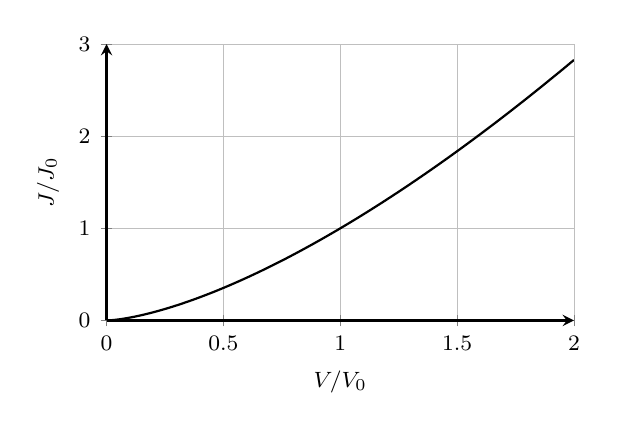
\begin{tikzpicture}
\begin{axis}[
 width=0.62\textwidth,
 height=0.42\textwidth,
 xlabel={$V/V_{0}$},
 ylabel={$J/J_{0}$},
 domain=0:2,
 samples=100,
 xmin=0, xmax=2,
 ymin=0, ymax=3,
 axis lines=left,
 thick,
 grid=both,
 grid style={line width=0.1pt, draw=gray!30},
 major grid style={line width=0.2pt, draw=gray!50},
 tick label style={font=\footnotesize},
 label style={font=\footnotesize},
]
\addplot[black, thick, domain=0:2, samples=100] {x^1.5};
\end{axis}
\end{tikzpicture}
\caption{Schematic, illustrative plot of the analytic Child--Langmuir scaling $J/J_{0} = (V/V_{0})^{3/2}$ of Eq.~\eqref{eq:annot:childlangmuir}. No experimental or simulated data are represented; the curve is included purely to fix the three-halves-power sheath scaling referenced throughout this appendix.}
\label{fig:annot:childlangmuir}
\end{figure}

\section{Methodological Synthesis}
\label{app:annot:synthesis}

The dependency structure linking the seven themes above runs strictly forward, since no single cited work spans the full chain from first-principles sheath theory to a validated erosion prediction. Section~\ref{app:annot:sheath-theory} fixes the boundary condition Eq.~\eqref{eq:annot:bohm} (or its magnetized form, Eq.~\eqref{eq:annot:bohmchodura}) that any admissible $f_{\mathrm{i}}(v)$ must satisfy at the sheath edge; Sec.~\ref{app:annot:ion-energy-flux} defines the moment of $f_{\mathrm{i}}(v)$, $\Gamma_{E}$ of Eq.~\eqref{eq:annot:gammaE}, the physically consequential output; Secs.~\ref{app:annot:lif-ivdf} and~\ref{app:annot:thomson} supply the two independent, non-perturbative measurement channels --- ion side and electron side --- from which $f_{\mathrm{i}}(v)$ and the boundary values entering Eq.~\eqref{eq:annot:bohm} are jointly constrained; Sec.~\ref{app:annot:inverse-problems} supplies the regularization apparatus, Eq.~\eqref{eq:annot:tikhonov}, without which neither channel's raw spectrum could be converted into an admissible estimate with defensible uncertainty; and Secs.~\ref{app:annot:hall-erosion} and~\ref{app:annot:fusion-pwi} close the loop by demonstrating, in two analogous settings, that $\Gamma_{E}$ so reconstructed governs the convex, threshold-sensitive surface response of Eq.~\eqref{eq:annot:erosion}. An error introduced at any stage --- an unmodelled deviation from Maxwellian electrons at the sheath-theory stage, or unaccounted broadening at the LIF stage --- therefore propagates multiplicatively rather than additively to the final prediction, because $\Gamma_{E}$ is a third-moment (velocity-cubed-weighted) integral of $f_{\mathrm{i}}(v)$ and is disproportionately sensitive to errors in the high-energy tail. This sensitivity is the principal justification for why an energy-\emph{resolved} estimator, rather than a mean-energy point estimate, is required wherever accurate erosion or heat-load prediction is the end goal.

\section{Summary}
\label{app:annot:summary}

The works annotated here trace a single continuous argument. The sheath-theory literature of Sec.~\ref{app:annot:sheath-theory} establishes the marginal ion speed $u_{\mathrm{B}}$ of Eq.~\eqref{eq:annot:bohm} and its kinetic, collisional, magnetized, and multi-species generalisations, fixing the boundary condition on $f_{\mathrm{i}}(v)$ at the sheath edge. Section~\ref{app:annot:ion-energy-flux} promotes this single-speed criterion to the full energy-resolved flux $\Gamma_{E}$ of Eq.~\eqref{eq:annot:gammaE}, the central quantity this monograph seeks to quantify. Sections~\ref{app:annot:lif-ivdf} and \ref{app:annot:thomson} supply the two principal non-perturbative diagnostic routes --- LIF for the ion side, Thomson scattering for the electron side --- while Sec.~\ref{app:annot:inverse-problems} supplies the regularization mathematics inverting noisy, line-integrated spectra into admissible profiles with quantified uncertainty. Finally, Secs.~\ref{app:annot:hall-erosion} and \ref{app:annot:fusion-pwi} demonstrate, in two analogous settings --- electric propulsion and magnetic confinement fusion --- that $\Gamma_{E}$, rather than the particle flux $\Gamma_{\mathrm{i}}$ alone, governs component erosion and lifetime via the threshold-like dependence expressed in Eq.~\eqref{eq:annot:erosion}. Read together, these seven themes justify both the theoretical construction and the diagnostic methodology this appendix supports.
